The primary aim of this research was to enable us to collect a series of probe
requests and process them into a usable pedestrian footfall count. We did this
by using a Wi-Fi receiver to collect probe requests broadcast by mobile devices,
filtering out the background noise, and aggregating them based on the device
that generated them. In this section, we examine the characteristics of probe
requests in detail, devise a methodology to collect these probe requests in
public areas, examine the systemic biases and uncertainties in the data
collection method, and devise data processing methods to overcome these
challenges. Finally, we compare the processed footfall counts to the ground
truth recorded by primary surveys.

Probe requests are a special type of management packet broadcast by Wi-Fi
enabled devices as part of their various functions such as scanning for
available APs and quick geolocation by triangulation based known APs, etc.
These are broadcast by all Wi-Fi enabled devices regardless of the manufacturer,
type or model of the devices, although there is some variation in the frequency
and the content of the information transmitted through them. In some cases, such
as Android devices, these are broadcast even when the Wi-Fi functionality has
been turned off by the user so that the device can immediately connect to
networks when the functionality is switched back on. Since some devices even use
the probe requests as a less accurate form of localisation, they continuously
send probe requests when Wi-Fi has been switched off. Thus, these signals can be
used to reliably identify the presence of Wi-Fi enabled mobile devices. Being a
first step of connection initiated by the mobile device, these packets have
information regarding the characteristics of the mobile device itself. Some of
the key information we can infer from these requests are,

\begin{enumerate} 
\item \textbf{Media Access Control (MAC) address} which is a name identifying
	the wireless hardware of the mobile device, 
\item \textbf{Sequence number} of the request for the mobile device to keep
	track of the responses, 
\item \textbf{Time stamp} at which the request was received by the AP, 
\item Total \textbf{length} of the request in number of bits, and 
\item The \textbf{strength of the signal} received by the mobile device.
\end{enumerate}

The MAC address is the primary identifier for the mobile device and has two
parts. The first part is the Organisationally Unique Identifier (OUI) which
provides information about the manufacturer of the device and the second part is
the identifier for the device. In modern devices, to protect users' privacy, the
second part of the MAC address can also be randomised and hence may not be
unique to devices. When the MAC address is randomised, it is marked as such by
setting a specific bit in the probe request packet as 1. Although sequence
number of the packet is strictly unique to a mobile device, we hypothesize that
we can use them to estimate the number of unique devices as demonstrated by
\citep{vanhoef2016}; where optional information present in the probe requests -
Information Elements (IE) along with the sequence numbers, have been used to
fingerprint the devices. This approach has become increasingly difficult as
mobile phone manufacturers have severely limited the IEs present in the probe
requests thus leading us to explore methods which use only the sequence numbers.
This also affects the established commercial solutions using Wi-Fi probe
requests such as Blix, Walkbase, Euclid Analytics, RetailNext etc.  There has
been another solution proposed by \citep{hong2018crowdprobe} where the authors
tried to solve the similar problem using a hidden markov models based trajectory
inference algorithm but the scope of this research was limited to enclosed, exit
controlled public spaces such as shopping malls, railway stations, etc.

Data collection was done with the help of custom sensors built from modifying
the hardware used in Smart Street Sensors \citep{sss2016} and updating them with
custom software. The sensor is essentially a Raspberry-Pi device with Wi-Fi and
3G modules. It keeps the Wi-Fi module in `Monitor mode' and uses the open source
software - Wireshark \citep{wireshark2} to passively collect all packets sent to
`broadcast', marked with type as `management', and subtype `probe requests'.
The MAC address in these probe requests is obfuscated at the device level using
a cryptographic hashing algorithm and transmitted through 3G connection to a
central database via web-sockets protocol, where it is stored in a PostgreSQL
database for further analysis. The random salt used in the hashing algorithm was
rotated regularly to further mitigate the risk of de-anonymisation of the hash.
Though hashing cannot completely ensure anonymisation as discussed in
\citep{demir2014analysing}, it can sufficiently obfuscate the data; which along
with a secure process of data handling, gives us reasonable security. An overall
schematic of the data collection and storage process is shown in Figure
\ref{datacollection_schematic}. The ground truth on the number of pedestrian
footfall was recorded using a custom Android application - Clicker
\citep{bala2018clicker}. This app logs accurate timestamps each time the
surveryor records a pedestrian crossing the designated cordon line at the
location. In addition to counting the pedestrians manually, this procedure
results in the device broadcasting probe requests regularly, which in turn,
gives us a `known device' to calibrate our methodology against.

\begin{figure} 
	\centering 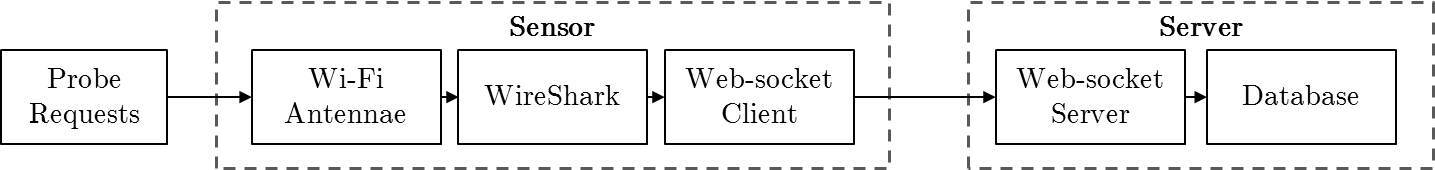
\includegraphics[width=\linewidth]
		{images/figure_1.jpeg}
	\caption 
		{Schematic diagram showing the process of collecting and storing probe
		requests using the sensor}
	\label{datacollection_schematic} 
\end{figure}

After collecting data, we began estimating the footfall or pedestrian activity
from them by identifying the following potential uncertainties arising from our
data collection method:

\begin{enumerate} 
\item 
\textbf{Background noise} - since the extent to which Wi-Fi signals travel
        differs subject to various factors such as interference and humidity, it
        is close to impossible to restrict our data collection to a finite area
        of interest. This can lead to a significant background noise at certain
        locations. For example, a phone shop or a bus stop located next to the
        study area can artificially increase the number of probe requests
        received by the sensor.  It is important to note that this method may
        not work effectively on study locations with complex configurations such
        as the source of noise and the area of study being located at the same
        distance from the sensor. This aspect is explored in detail in the
        broader case study in the following sections.
\item 
\textbf{MAC randomisation} - mobile devices in recent years have been using
        randomised `local' MAC addresses for probe requests to protect the users
        from being tracked. This makes it impossible to tell if the probe
        requests are being sent by the same mobile device. This along with the
        previous problem can further increase the magnitude of error by several
        fold.
\item
\textbf{Mobile ownership} - since the rate of mobile ownership can vary widely
		across geography and demography, we cannot assume that every mobile
		device translates to one pedestrian footfall. In addition to this, there
		is a long term overall increase in mobile ownership which may affect 
		the number of probe requests collected overtime.
\end{enumerate}

We propose the following internal and external validation methods to tackle each
of these uncertainties.

\begin{figure} 
\centering 
\subfigure [Distribution of signal strengths (dBm) showing the filtering of
		background noise] {\resizebox*{0.45\linewidth}{!}
		{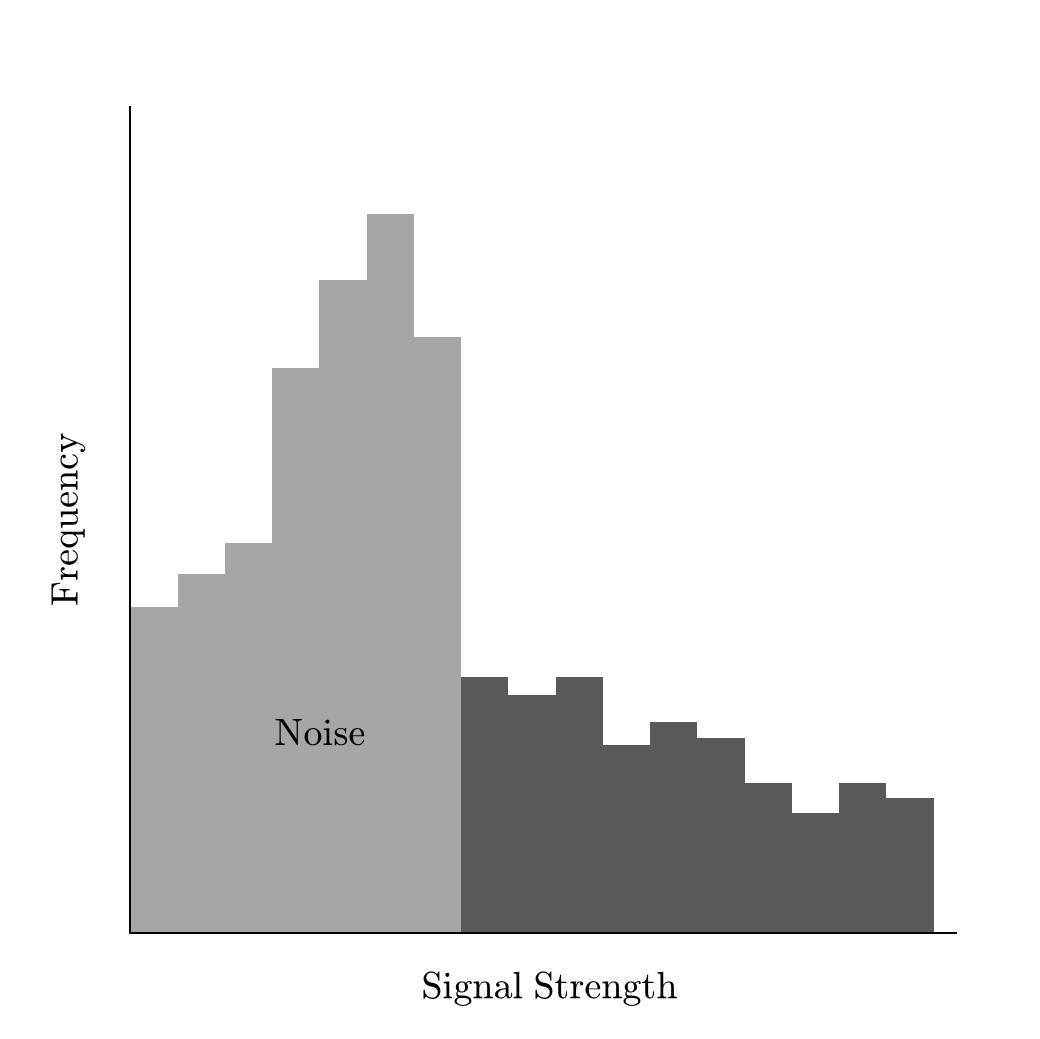
\includegraphics{images/figure_2a.jpeg}}}
\hspace{20pt}
\subfigure [Clustering probe requests as nodes in a graph using increasing
		sequence numbers] {\resizebox*{0.45\linewidth}{!}
		{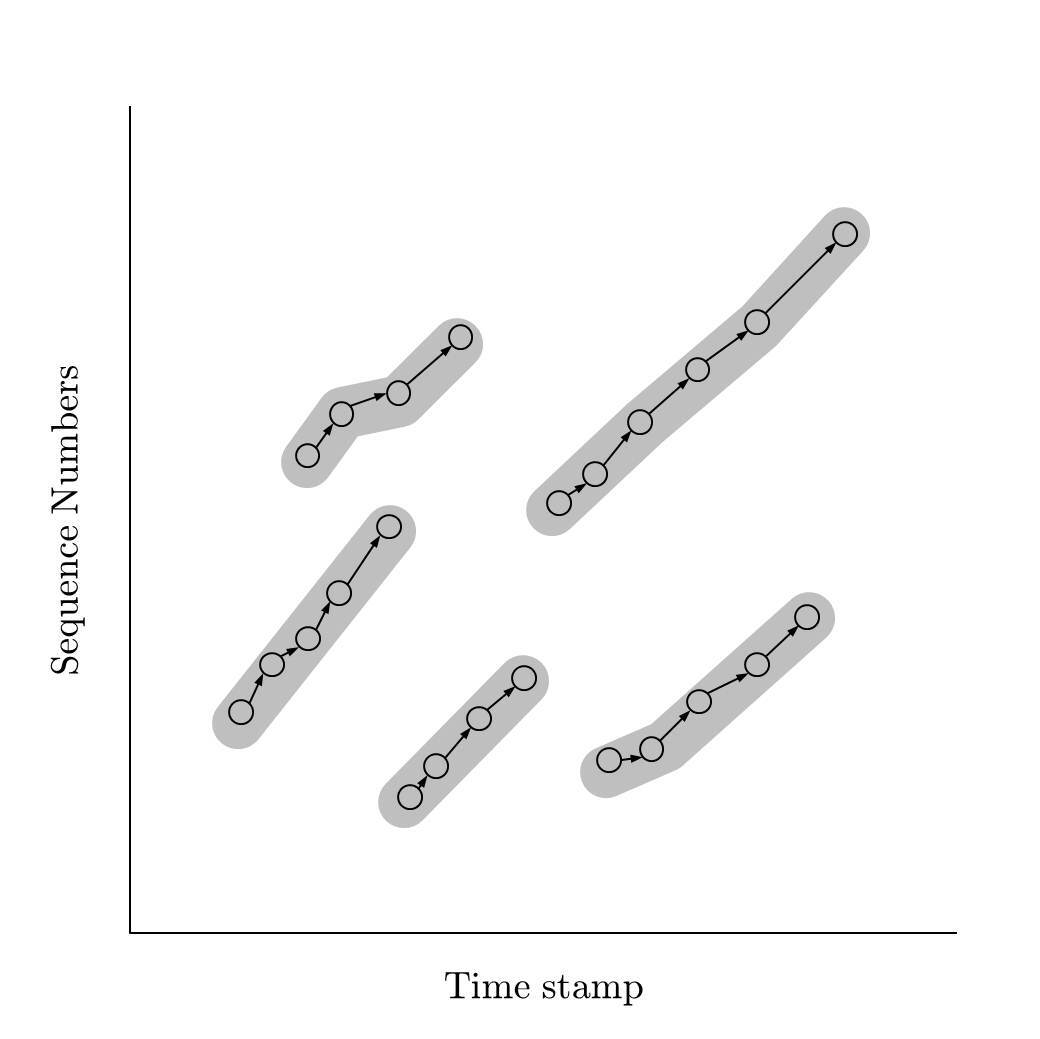
\includegraphics{images/figure_2b.jpeg}}}
\caption {Schematic diagrams explaining the methods for filtering by signal
	strength and clustering using sequence numbers}
\label{methodology_schematic}
\end{figure}

\subsection{Filtering with Signal Strength} 

One of the clues that we can use to estimate the distance between the mobile
device and the sensor is the strength of the signal received by the sensor. The
obvious approach was to first try and establish a relationship between the
signal strength and distance and to use this to filter out the unwanted probe
requests. However this approach was found to not be feasible, since the decay of
signal strength with respect to distance is not always constant. For instance,
signal strength varies with atmospheric conditions, the presence of obstructions
between the source and the target, the nature of these obstructions, and the
strength (power level) of the source. This severely limits our ability to
establish a simple conversion between reported signal strength and distance. As
such, there was a need for a method which takes in to account all of these
variables across the various locations.

We assumed that, in configurations where a specific source of background noise
was at a constant distance, there must be a distinct pattern in the number of
probe requests reporting signal strength corresponding to that distance. For
example, if there was a phone shop next to our sensor where hundreds of phones
regularly sent probe requests, there should be a sharp rise in the of number of
probe requests with reported signal strength corresponding to the distance
between the sensor and the phone shop, irrespective of the local conditions as
shown in Figure \ref{methodology_schematic}. We could identify these breaks in
the data using traditional one dimensional clustering algorithms such as `jenks
natural breaks', `k-means', `quantile' and `hierarchical clustering', etc. Since
we were only looking for the break in the data and not for absolute values, the
methodology should apply for all the variations due to micro site conditions
reducing the overall noise in the collected data.

\subsection{Clustering with sequence numbers}

Since our primary unique identifier - MAC addresses are being anonymised by new
devices, we needed to find other information present in the probe requests for
use as a unique identifier. The obvious approach was to establish a factor of
randomisation, and adjust the counts for the probe requests based on this
factor. We found this approach to not be feasible since the proportion of
devices which randomise the MAC addresses increased over time. There was also a
wide variation in the frequency at which the devices randomised the MAC
addresses and the method used for the process. This led us to look for a more
generalisable approach which was independent of the device model.

From our initial look at the data, we found that OUI and the sequence number of
the packet was the most promising information to achieve this.  First we divided
our dataset into sets of probe requests with randomised and non-randomised MAC
addresses by looking at the second character of the vendor part of the MAC
address; if it was E, A, 2 or 6, then those addresses were identified to be
randomised. We kept the MAC address as the unique identifier for the
non-randomised requests and further divided the randomised ones in to
sub-categories based on their OUI. We then  identified unique mobile devices
from within those sets, and assigned a unique identifier to each device.

The proposed algorithm created a graph where the probe requests represented the
nodes; links were created between them based on the following rules:

\begin{itemize} 
\item A link could go only forward in time. 
\item A link could go from low to high sequence numbers. 
\item A link could exist between nodes with a maximum time difference of
	$\alpha$ - time threshold. 
\item A link could exist between nodes with a maximum sequence number
	difference of $\beta$ - sequence threshold.
\item A node could have only one incoming link and one outgoing link, which is
	the shortest of all such possible links in terms of both time and sequence
	number.
\end{itemize}

The nodes were then assigned a unique ID based on the unique connected component
they belonged to as shown in Figure \ref{methodology_schematic}. This unique
identifier was used in the place of MAC addresses for aggregation of the
anonymised probe requests. Although the recycling of sequence numbers after 4096
led to multiple unique IDs being reported from a single device, a sample
consisting of all randomised probe requests sent by "Google" devices showed that
only 0.5\% of the sample had their sequence number reset. This led assume this
to be inconsequential. 

\subsection{Calibrating with Ground Truth} 

Since proportions of mobile device ownership was an external uncertainty to our
study and could arise from variety of spatio - temporal and demographic factors,
we aimed to solve this by using a manual sample count at each location. We then
calculated an adjustment factor, or an `offset' for each location by comparing
the sensor-based counts and ground truth. In turn it was then used to adjust the
data reliably to reflect the ground truth in absolute numbers.  This calibration
can be carried out periodically at these locations to improve the quality of the
estimation.
